\documentclass{article}

\usepackage{tikz} 
\usetikzlibrary{automata, positioning, arrows} 

\usepackage{amsmath}
\usepackage{amsthm}
\usepackage{amsfonts}
\usepackage{amsmath}
\usepackage{amssymb}
\usepackage{fullpage}
\usepackage{color}
\usepackage{parskip}
\usepackage{graphicx}
\usepackage{hyperref}
  \hypersetup{
    colorlinks = true,
    urlcolor = blue,       % color of external links using \href
    linkcolor= blue,       % color of internal links 
    citecolor= blue,       % color of links to bibliography
    filecolor= blue,        % color of file links
    }
    
\usepackage{listings}

\definecolor{dkgreen}{rgb}{0,0.6,0}
\definecolor{gray}{rgb}{0.5,0.5,0.5}
\definecolor{mauve}{rgb}{0.58,0,0.82}

\lstset{frame=tb,
  language=haskell,
  aboveskip=3mm,
  belowskip=3mm,
  showstringspaces=false,
  columns=flexible,
  basicstyle={\small\ttfamily},
  numbers=none,
  numberstyle=\tiny\color{gray},
  keywordstyle=\color{blue},
  commentstyle=\color{dkgreen},
  stringstyle=\color{mauve},
  breaklines=true,
  breakatwhitespace=true,
  tabsize=3
}

\newtheoremstyle{theorem}
  {\topsep}   % ABOVESPACE
  {\topsep}   % BELOWSPACE
  {\itshape\/}  % BODYFONT
  {0pt}       % INDENT (empty value is the same as 0pt)
  {\bfseries} % HEADFONT
  {.}         % HEADPUNCT
  {5pt plus 1pt minus 1pt} % HEADSPACE
  {}          % CUSTOM-HEAD-SPEC
\theoremstyle{theorem} 
   \newtheorem{theorem}{Theorem}[section]
   \newtheorem{corollary}[theorem]{Corollary}
   \newtheorem{lemma}[theorem]{Lemma}
   \newtheorem{proposition}[theorem]{Proposition}
\theoremstyle{definition}
   \newtheorem{definition}[theorem]{Definition}
   \newtheorem{example}[theorem]{Example}
\theoremstyle{remark}    
  \newtheorem{remark}[theorem]{Remark}

\title{CPSC-354 Report}
\author{Gabriel Davidson  \\ Chapman University}

\date{\today} 

\begin{document}

\maketitle

\begin{abstract}
This report examines the progression of concepts within the umbrella of programming languages theory through 13 of weeks of theory-driven lecture, homework, and assignments. The driving concepts are lambda calculus and associated content, especially with respect to theorems and proofs, recursion as a programming strategy, parsing theory and its applications on interpreted languages, and context free grammars and the parsing of input into abstract syntax trees. We implemented the theory learned in class into 4 programming assignments that built off of each other to explore foundational topics, especially recursion, context-free grammars, abstract syntax trees, and the implementation of interpreters for custom languages. The final assignment culminates with an interpreter capable of handling complex operations, including conditional logic, variables, if-then-else blocks, lists, and recursive functions. Through these assignments, and through exercises practicing concepts core to the class's curriculum, how to implement meaningful concepts into concrete behaviour. 
\end{abstract}

\setcounter{tocdepth}{3}
\tableofcontents

\section{Introduction}\label{intro}
Programming languages serve as the basis for computer science and enable the expression of complex behaviour, systems, and problems into executable programs. Languages allow develops to take on these problems, just as spoken languages allow humans to express themselves, by providing syntax and semantics. The theory behind programming languages is a huge canvas of concept and topics, and in this class we take on understanding the role of lambda calculus and its associated content, parsing theory, and context free grammars, among others. These topics are central to understanding the origins of programming languages as written languages, and also to designing and implementing custom languages of our own.

This report will focus on that journey, from proving the validity of logic programs to creating our own context free grammars. By integrating theory with practical implementations, this course has taught me how abstract ideas can translate into tangible behaviour, and how we can utilize that behaviour to capture the essence of written syntax and transform (interpret!) it into executable logic.
\section{Week by Week}\label{homework}

\subsection{Week 1}

\subsubsection*{Notes}
This week in class we mainly focused on learning Lean, setting up \LaTeX, and a brief lecture on the basis of $Proof = Program$. This idea shows how logical mathematical proofs are a constructive process, building on previously founded theorems and definitions. This idea transfers to theoretical programming in the sense that programs are also constructed proofs. The execution of a program is the execution of many logical steps in a proof. I enjoy how this relates to the "human" process as well - our activities are the execution of previously learned strategies in a logical way.

\subsubsection*{Question} I was interested in learning more about Proof = Program, and some additional sleuthing showed me how a running a program is simply executing the steps in a logical proof. I was wondering how more complex program design methods such as recursion adhere to this idea, and if there are other programming methodologies that do not adhere to Proof = Program?

\subsubsection*{Homework}

  \subsubsection*{Level 5 - Adding Zero}
  In this level we prove the theorem that $\textbf{a+0=a}$ using $\textbf{a+(b+0)+(c+0)=a+b+c}$. Here is how I solved this theorem.

  \bgroup\obeylines
  \qquad \textbf{repeat rw add zero}
  \qquad \textbf{rfl}
  \egroup

  \subsubsection*{Level 6 - Adding Zero}
  In this level we built on the solution from the previous level to learn how to use precision rewriting.

  \bgroup\obeylines
  \qquad \textbf{rw add zero c}
  \qquad \textbf{repeat rw add zero}
  \qquad \textbf{rfl}
  \egroup

  \subsubsection*{Level 7 - Add Suc}
  In this level we prove the theorem that $\textbf{succ(a)=a+1}$.

  \bgroup\obeylines
  \qquad \textbf{rw one eq add zero}
  \qquad \textbf{repeat rw add zero}
  \qquad \textbf{rfl}
  \egroup

  \subsubsection*{Level 8 - Add Suc}
  In this level we prove the equation that $\textbf{2+2=4}$. This was the final level in the Tutorial World, and required the accumulation of definitions and theorems learned so far. I will provide the assumptions that I used when deciding my proof in Lean.

  \bgroup\obeylines
  \qquad \textbf{rw four eq succ three} —— Any number $n = succ(pred(n))$
  \qquad \textbf{rw three eq succ two}  —— Any number $n = succ(pred(n))$
  \qquad \textbf{rw two eq succ one}    —— Any number $n = succ(pred(n))$
  \qquad \textbf{rw one eq succ zero}   —— Any number $n = succ(pred(n))$
  \qquad \textbf{repeat rw add succ}    —— Using $a + succ b = succ (a + b)$
  \qquad \textbf{rw add zero}           —— Using $a + 0 = a$
  \qquad \textbf{rfl}                   —— Proves the goal $X = X$

  \egroup

%In case you want to draw automata in Latex, you can use the tikz %package. Here is an example of a simple automaton:
%
%\begin{tikzpicture}[shorten >=1pt,node distance=2cm,on grid,auto] 
%  \node[state] (q_1)   {$q_1$}; 
%  \node[state] (q_2) [above right=of q_1] {$q_2$}; 
%  \node[state] (q_3) [below right=of q_2] {$q_3$}; 
%   \path[->] 
%   (q_1) edge  node {0} (q_2)
%         edge  node [swap] {1} (q_3)
%   (q_2) edge  node  {1} (q_3)
%         edge [loop above] node {0} ()
%   (q_3) edge [loop below] node {0,1} ();
%\end{tikzpicture}
%
%By the way, GPT-4 is quite good at outputting tikz code.

\subsubsection*{Comments and Questions}

%(Delete and Replace:) Here you should write your own critical reflection on the content of the week. If you can surprise me with something I have not seen before, you are on the right track.

%I expect you to read the lecture notes. 

Ask at least one \textbf{interesting question}\footnote{It is important to learn to ask \emph{interesting} questions. There is no precise way of defining what is meant by interesting. You can only learn this by doing. An interesting question comes typically in two parts. Part 1 (one or two sentences) sets the scene. Part 2 (one or two sentences) asks the question. A good question strikes the right balance between being specific and technical on the one hand and open ended on the other hand. A question that can be answered with yes/no is not an interesing question.} on the lecture notes. Also post the question on the Discord channel so that everybody can see and discuss the questions.

\subsection{Week 2}

\subsubsection*{Notes}
Translating Lean into Math by matching each line in Lean to the corresponding mathematical equation and assumptions. Being able to reverse the proof and translate from Math into Lean is also important. Lean reads from the goal to the axioms, whereas Math is written from the axioms to the goal (usually).
\newline \newline Defining data types recursively (in terms of itself). Syntax varies by language. 
\newline \newline Recursion example with the Tower of Hanoi. Breaking logical puzzles into iterative steps, then into recursive steps.

\subsubsection*{Question}
In class we used recursion to prove an algorithmic solution for the tower of hanoi game. Within the scope of proofs, what are the biggest drawbacks/advantages to using iterative vs recursive techniques?

%(Delete:) Week 2 (and all the other weeks) should follow the same pattern as Week 1. Even if there is a week without homework, notes and comments (see above) are still expected.

\subsubsection*{Homework}

\subsubsection*{Level 1 - Zero Add}
  In this level we prove the theorem that $\textbf{0 + n = n}$. It was our first use of proof by induction.

  \bgroup\obeylines
  \qquad \textbf{induction n with d hd}
  \qquad \textbf{rw add zero}
  \qquad \textbf{rfl}
  \qquad \textbf{rw add succ}
  \qquad \textbf{rw hd}
  \qquad \textbf{rfl}
  \egroup

  \subsubsection*{Level 2 - Succ Add}
  In this level we prove the theorem that $\textbf{succ(a) + b = succ(a + b)}$.

  \bgroup\obeylines
  \qquad \textbf{induction b with d hd}
  \qquad \textbf{repeat rw add zero}
  \qquad \textbf{rfl}
  \qquad \textbf{rw add succ}
  \qquad \textbf{rw hd}
  \qquad \textbf{rw add succ}
  \qquad \textbf{rfl}
  \egroup

  \subsubsection*{Level 3 - Add Comm}
  In this level we prove the theorem that $\textbf{a + b = b + a}$.

  \bgroup\obeylines
  \qquad \textbf{induction b}
  \qquad \textbf{rw add zero}
  \qquad \textbf{rw zero add}
  \qquad \textbf{rfl}
  \qquad \textbf{rw succ add}
  \qquad \textbf{rw add succ}
  \qquad \textbf{rw nih}
  \qquad \textbf{rfl}
  \egroup

  \subsubsection*{Level 4 - Add Assoc}
  In this level we prove the theorem that $\textbf{(a + b) + c = a + (b + c)}$.

  \bgroup\obeylines
  \qquad \textbf{induction b}
  \qquad \textbf{rw add zero}
  \qquad \textbf{rw zero add}
  \qquad \textbf{rfl}
  \qquad \textbf{rw add succ}
  \qquad \textbf{rw succ add}
  \qquad \textbf{rw nih}
  \qquad \textbf{rw add comm}
  \qquad \textbf{rw succ add}
  \qquad \textbf{rw add succ}
  \qquad \textbf{rfl}
  \egroup

  \subsubsection*{Level 5 - Add Comm Right}
  In this level we prove the theorem that $\textbf{(a + b) + c = (a + c) + b}$. I will show the mathematical assumptions I used when deciding my proof in Lean.

  \bgroup\obeylines
  \qquad \textbf{rw add assoc a b} —— (RHS) By associativity rule, $\textbf{a + c + b = a + (c + b)}$
  \qquad \textbf{rw add assoc} —— (LHS) By associativity rule, $\textbf{a + b + c = a + (b + c)}$
  \qquad \textbf{rw add comm b c} —— (LHS) By commutative rule, $\textbf{a + (b + c) = a + (c + b)}$
  \qquad \textbf{rfl} —— Proves the goal $\textbf{X = X}$
  \egroup

\subsection{Week 3}

\subsubsection*{Notes}
This week we talked a lot about context free grammars, especially within the context of parsing mathematical expressions. I really enjoyed learning more about CFGs, especially visualized, because it helped me to understand how CFGs are so important for programming languages. I also couldn't help but think how cool the visualized abstract syntax tree was. It makes me think more about how this sort of approach can be applied to other areas. I had unintentionally started designing my calculator using a similar paradigm, recursively splitting the expression into two small parts until each expression was complete. (I ended up switching approaches, but I thought it was cool anyway).

I was doing some additional research into ASTs, and was intrigued by the subsequent processes also required as part of compilation. Semantic analysis, for example. How many other steps are necessary for compilation? Does this process change for interpreted languages? I would be interested in learning more about the overhead costs of script compilation.

\subsubsection*{Question} Last week we talked about context free grammars, especially within the context of mathematical syntax. Reading online, I learned about context-sensitive grammars. Can a CFG also be described as a CSG, or vice-versa? From what I could tell online, CSGs are invariably more complex than CFGs, so are there any actual applications of context sensitive grammars, and how is this reflected in its AST?

\subsubsection*{Homework}
\begin{center}
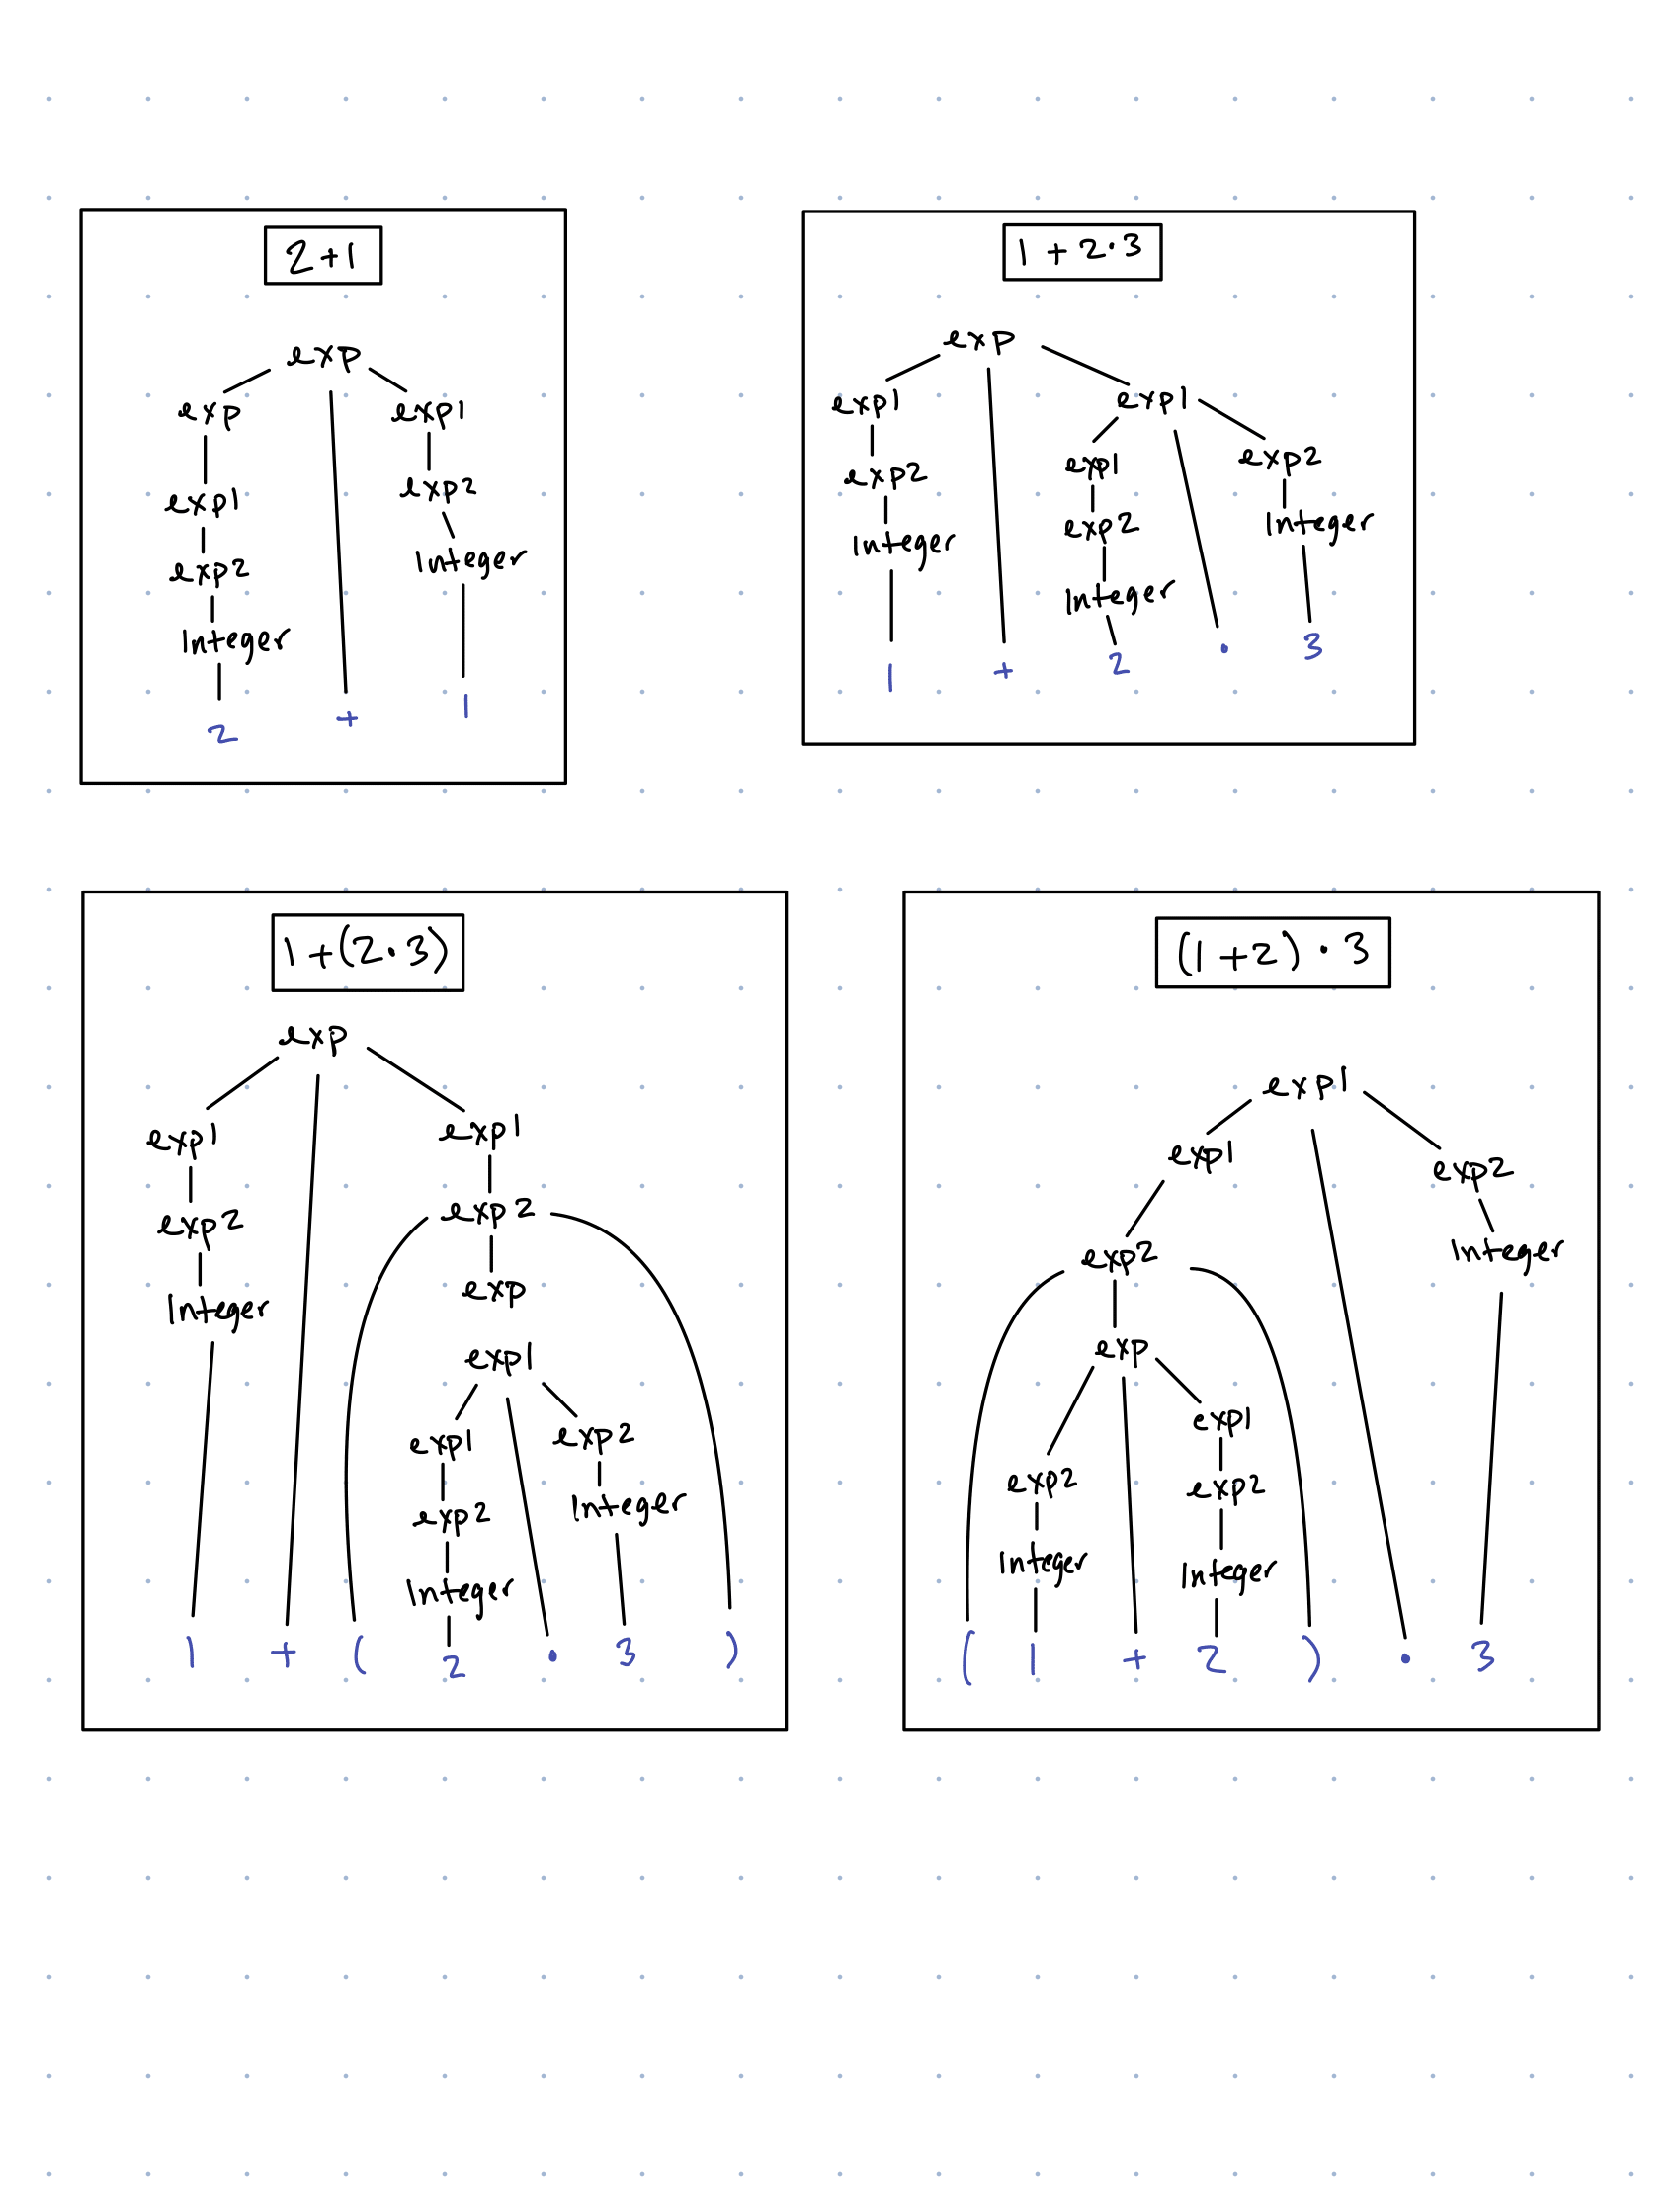
\includegraphics[scale=.5]{CPSC354 HW4-1.png}
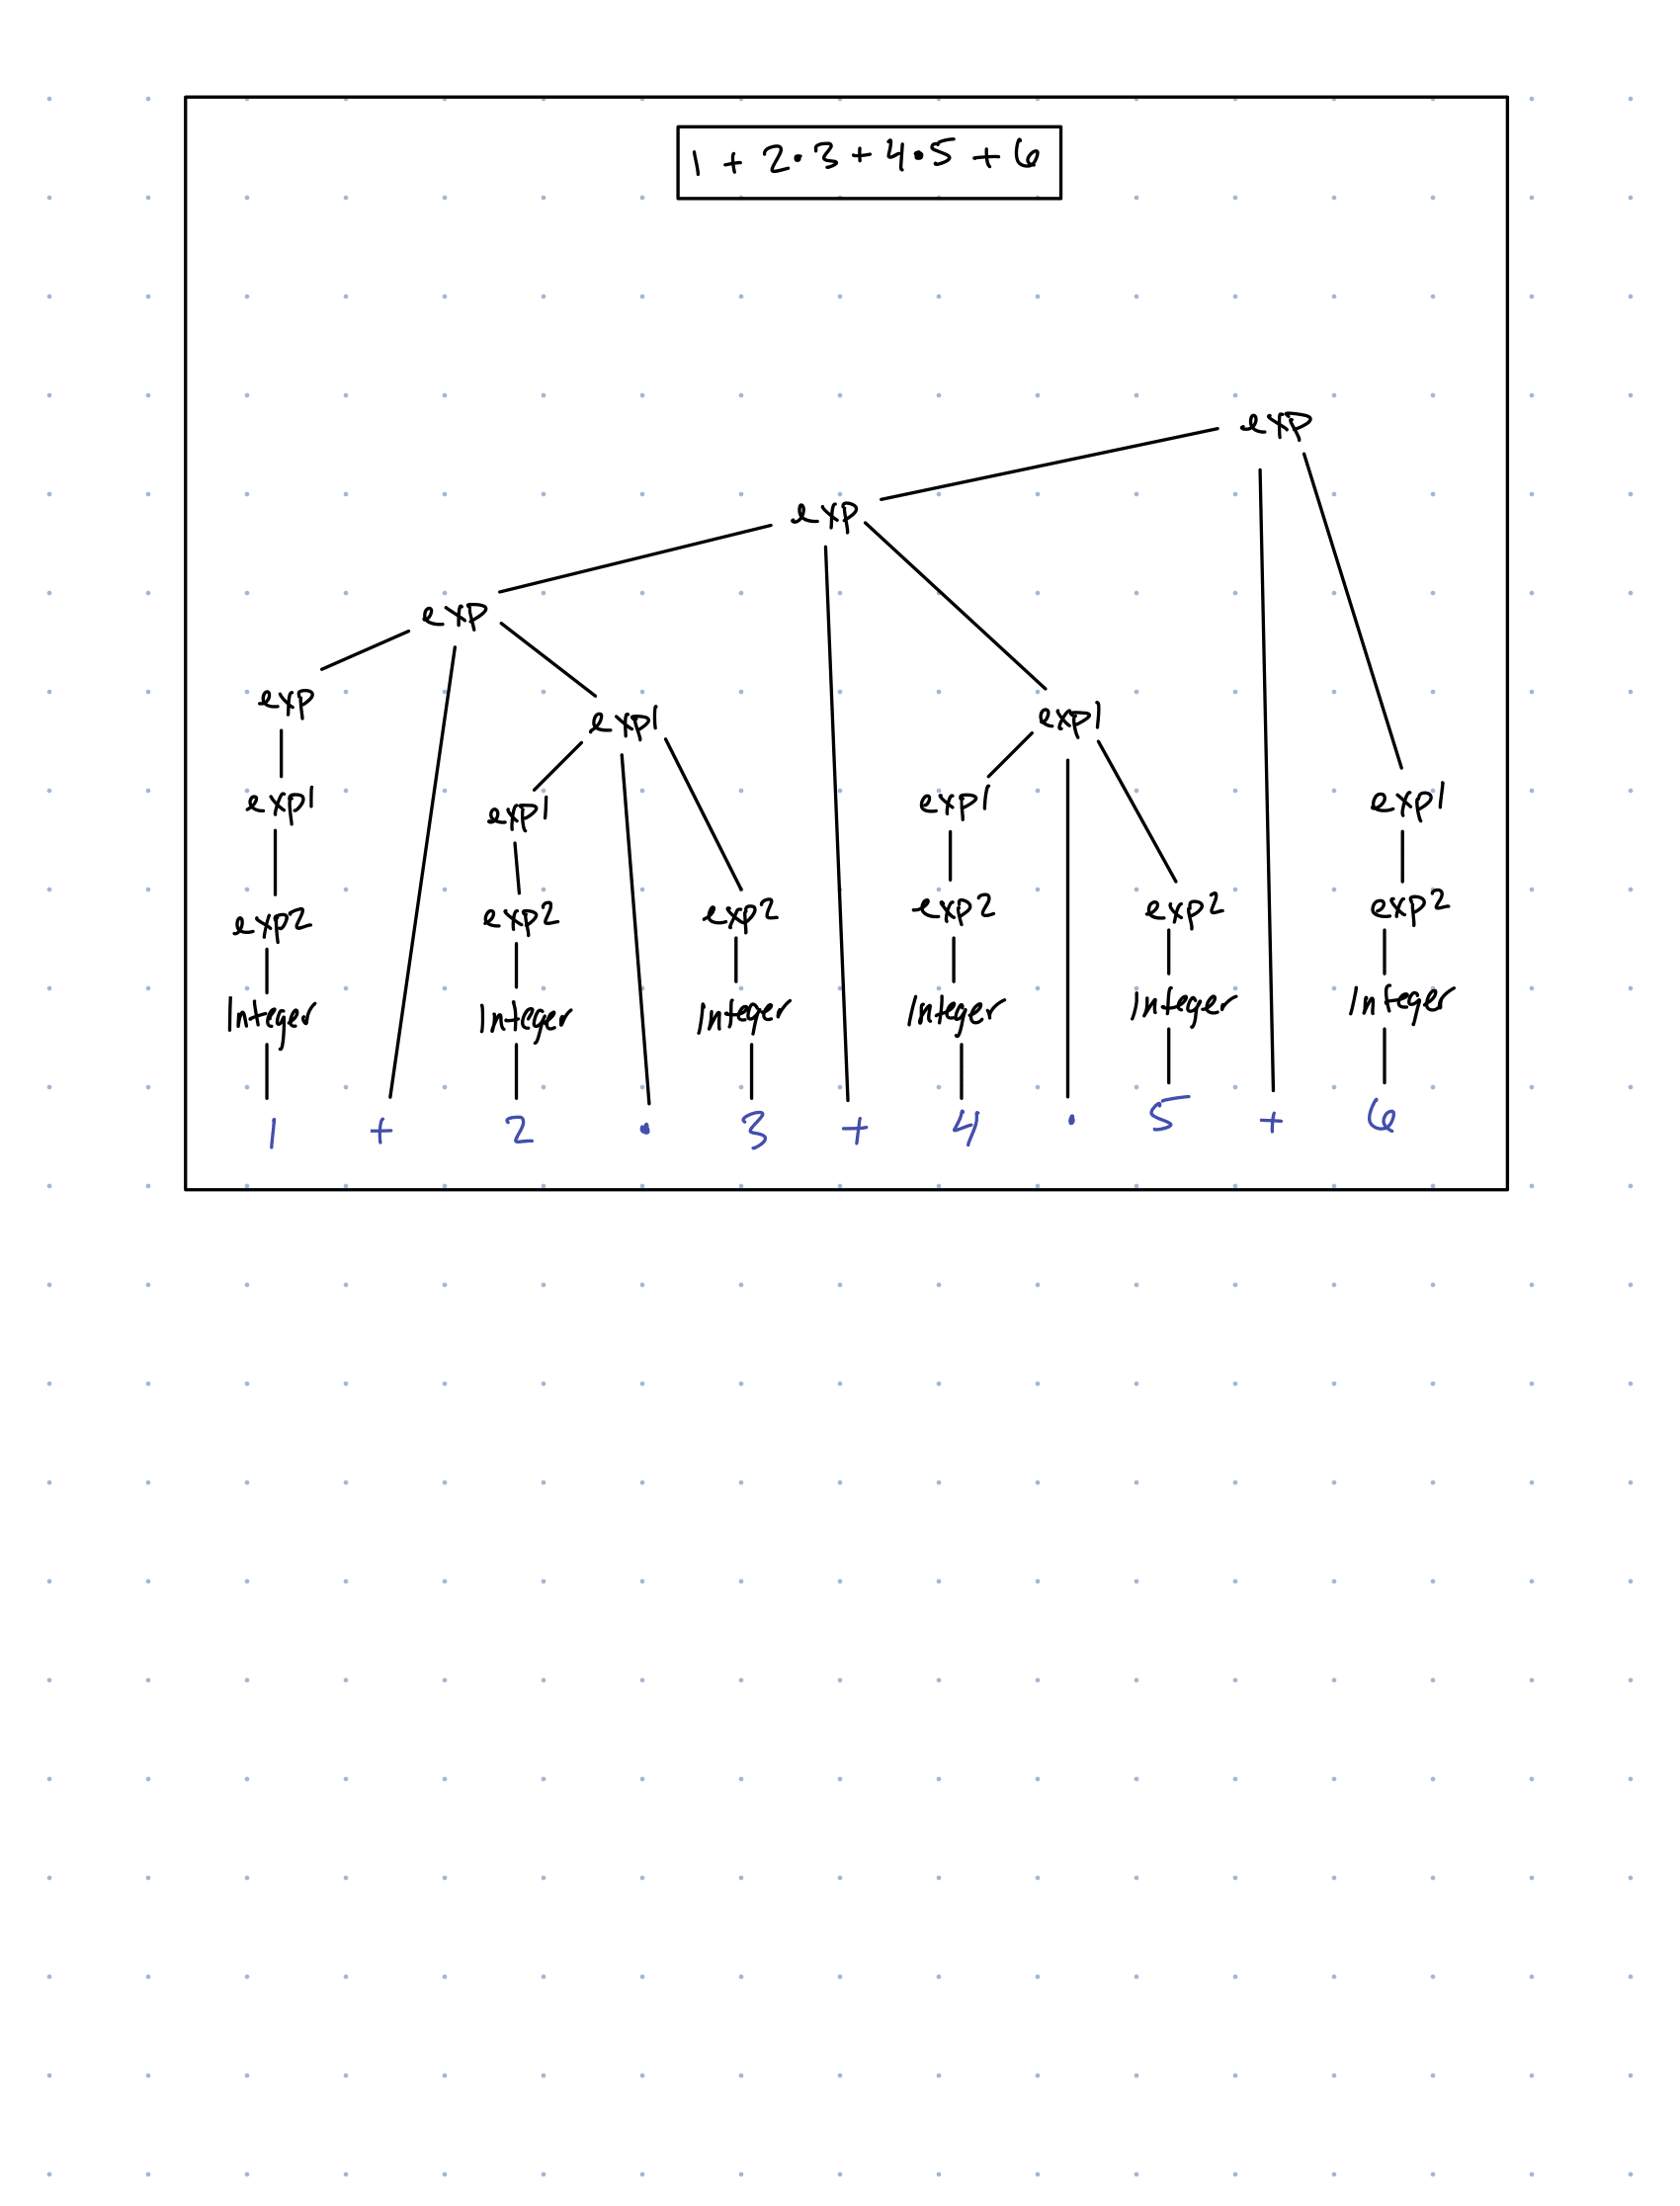
\includegraphics[scale=.6]{CPSC354 HW4-2.png}
\end{center}

\subsection{Week 4}

\subsubsection*{Notes} This week we discussed creating a calculator with CFGs and then about the next Lean world on logic. The logic world, similar to the math world, is about breaking down larger problems into manageable parts and tackling them one by one. If we can prove every infitessimal aspect of a larger problem, then we solve that large problem. I have really enjoyed working in the logic world so far because it is very similar to code design in game development. In game development, there are a number of components that control more context specific components, from the most high-level management context to the most basic mechanic. 

\subsubsection*{Question} Similar to Lianal's question, why does the logic world in Lean allow for varying syntax, while the math Lean world did not? Is this reflected in real (written) math/logic proofs?

\subsubsection*{Homework}

\subsubsection*{Level 1 - Exactly! It's in the premise}
Assumptions: $(P : Prop)(todo\_list : P) : P := by$

\[
\begin{aligned}
  (1)&\text{ exact todo\_list}
\end{aligned}
\]

\subsubsection*{Level 2 - And Introduction}
Assumptions: $(P S : Prop)(p: P)(s : S) : P \wedge S := by$

\[
\begin{aligned}
  (1)&\text{ exact ⟨ p, s ⟩}
\end{aligned}
\]

\subsubsection*{Level 3 - The Have Tactic}
Assumptions: $(A I O U : Prop)(a : A)(i : I)(o : O)(u : U) : (A \wedge I) \wedge O \wedge U := by$

\[
\begin{aligned}
  (1)& \text{ have ai } \text{:= and\_intro a i}\\
  (2)& \text{ have ou } \text{:= and\_intro o u}\\
  (3)& \text{ exact ⟨ ai, ou ⟩}
\end{aligned}
\]

\subsubsection*{Level 4 - And Elimination}
Assumptions: $(P S : Prop)(vm: P \wedge S) : P := by$

\[
\begin{aligned}
  (1)& \text{ have p } \text{:= vm.left}\\
  (2)& \text{ exact p}
\end{aligned}
\]

\subsubsection*{Level 5 - And Elimination 2}
Assumptions: $(P Q : Prop)(h: P \wedge Q) : Q := by$

\[
\begin{aligned}
  (1)& \text{ have q } \text{:= h.right}\\
  (2)& \text{ exact q}
\end{aligned}
\]

\subsubsection*{Level 6 - Mix and Match}
Assumptions: $(A I O U : Prop)(h1 : A \wedge I)(h2 : O \wedge U) : A \wedge U := by$

\[
\begin{aligned}
  (1)& \text{ exact ⟨ h1.left, h2.right ⟩ }
\end{aligned}
\]

\subsubsection*{Level 7 - More Elimination}
Assumptions: $(C L : Prop)(h: (L \wedge (((L \wedge C) \wedge L) \wedge L \wedge L \wedge L)) \wedge (L \wedge L) \wedge L) : C := by$

\[
\begin{aligned}
  (1)& \text{ exact h.left.right.left.left.right }
\end{aligned}
\]

\subsubsection*{Level 8 - Rearranging Boxes}
Assumptions: $(A C I O P S U : Prop)(h: ((P \wedge S) \wedge A) \wedge \neg I \wedge (C \wedge ¬O) \wedge ¬U) : A \wedge C \wedge P \wedge S := by$

\[
\begin{aligned}
  (1)& \text{ have c } \text{:= h.right.right.left.left}&\\
  (2)& \text{ have psa } \text{:= h.left}&\\
  (3)& \text{ have p } \text{:= psa.left.left}&\\
  (4)& \text{ have s } \text{:= psa.left.right}&\\
  (5)& \text{ have a } \text{:= psa.right}&\\
  (6)& \text{ exact ⟨ a, c, p, s ⟩ }
\end{aligned}
\]

\subsection{Week 5}

\subsubsection*{Notes} This week we discussed lambda higher order functions 
in the context of Lambda functions and had an interesting discussion about Curry 
Howard correspondance (currying) and languages. Lambda calculus functions are nameless, 
type-free functions. Within the context of lean, at least, this has been a difficult concept 
to grasp, because it is antithetical to the programming philosophy I have learned and practiced. 
However, the nature of lambda calculus is the same, but instead of relying on type-specific context, 
it relies on underlying logic within implicic type-deriving and preservation. I think this was 
confusing to me also because it throws explicit type safety out the window. On Thursday we discussed 
currying, $\alpha$-Conversion, $\beta$-Reduction, (and more) and had an interesting discussion about languages, 
and meaning behind language.  

\subsubsection*{Question} How do modern programming languages utilize (or avoid) lambda calculus in their syntax? In C\#, linq utilizes higher order functions encapsulating (what appears to be) explicitly defined lambda calculus functions, for example "enum.Where(x $\Rightarrow$ x.a $>$ 10)". It also seems like SQL syntax follows currying of lambda calculus functions, for example "SELECT * FROM \_ WHERE \_ ORDER BY \_", despite SQL not being a functional programming language.

\subsubsection*{Homework}

\subsubsection*{Level 1 - Cake Delivery Service}
Assumptions: $(P C: Prop)(p: P)(bakery\_service : P \rightarrow C) : C := by$

\[
\begin{aligned}
  (1)&\text{ exact (bakery\_service p)}
\end{aligned}
\]

\subsubsection*{Level 2 - Identity}
Assumptions: $(C: Prop) : C \rightarrow C := by$

\[
\begin{aligned}
  (1)& \text{ exact } \lambda \text{ var } \mapsto \text{ var }
\end{aligned}
\]

\subsubsection*{Level 3 - Cake Form Swap}
Assumptions: $(I S: Prop) : I \wedge S \rightarrow S \wedge I := by$

\[
\begin{aligned}
  (1)& \text{ exact } \lambda \text{ h : I } \wedge \text{ S } \mapsto \text{ and\_intro h.right h.left }
\end{aligned}
\]

\subsubsection*{Level 4 - And Elimination}
Assumptions: $(C A S: Prop) (h1 : C \rightarrow A) (h2 : A \rightarrow S) : C \rightarrow S := by$

\[
\begin{aligned}
  (1)& \text{ exact } \lambda \text{ c } \mapsto \text{ h2 (h1 c) }
\end{aligned}
\]

\subsubsection*{Level 5 - Riffin Snacks}
Assumptions: $(P Q R S T U: Prop) (p : P) (h1 : P \rightarrow Q) (h2 : Q \rightarrow R) (h3 : Q \rightarrow T) (h4 : S \rightarrow T) (h5 : T \rightarrow U) : U := by$

\[
\begin{aligned}
  (1)& \text{exact h5 (h3 (h1 p))}
\end{aligned}
\]

\subsubsection*{Level 6 - and\_imp}
Assumptions: $(C D S: Prop) (h : C \wedge D \rightarrow S) : C \rightarrow D \rightarrow S := by$

\[
\begin{aligned}
  (1)& \text{ exact } \lambda \text{ c d } \mapsto \text{ h (and\_intro c d) }
\end{aligned}
\]

\subsubsection*{Level 7 - and\_imp 2}
Assumptions: $(C D S: Prop) (h : C \rightarrow D \rightarrow S) : C \wedge D \rightarrow S := by$

\[
\begin{aligned}
  (1)& \text{ exact } \lambda \text{ ⟨c, d⟩ } \mapsto \text{ h c d }
\end{aligned}
\]

\subsubsection*{Level 8 - Distribute}
Assumptions: $(C D S : Prop) (h : (S \rightarrow C) \wedge (S \rightarrow D)) : S \rightarrow C \wedge D := by$

\[
\begin{aligned}
  (1)& \text{ have ⟨l, r⟩ := h}\\
  (2)& \text{ exact } \lambda \text{ s } \mapsto \text{ ⟨l s, r s⟩ }
\end{aligned}
\]

\subsubsection*{Level 9 - Uncertain Snacks}
Assumptions: $(R S : Prop) : R \rightarrow (S \rightarrow R) \wedge (\neg S \rightarrow R) := by$

\[
\begin{aligned}
  (1)& \text{ exact } \lambda \text{ r } \mapsto \text{ and\_intro ( } \lambda \text{ \_ } \mapsto \text{ r ) } \lambda \text{ \_ } \mapsto \text{ r}
\end{aligned}
\]

\subsection{Week 6}

\subsubsection*{Notes} This week we dove into theory discussions and lectures on application of currying, more complex lambda calculus and church numerals. To be honest, it is hard to remember much notes-wise because the theory was so intense, but I can say with confidence that I was confused - and embraced it! To help with my understanding, I looked for resources online and found this paper by Helmut Brandl titled \textbf{Limits of Computability in Lambda Calculus} (\url{https://hbr.github.io/Lambda-Calculus/computability/text.html}) which actually covered nicely what we have been learning about recently. In the preamble, Kurt Goedel's \textit{Godel Numbering} is discussed, and I thought the paper gave some interesting historical context to a memorable moment in logic and maths history; "In his famous incompleteness theorem (1931) Goedel demonstrated that paradoxical statements can be injected into all formalisms which are powerful enough to express basic arithmetics." Anyway, I digress. 

\subsubsection*{Question} Since lambda calculus is comprised of only abstraction and application, and cannot examine itself, how can infinitely recursing expressions like $(\lambda x.xx)(\lambda x.xx)$ terminate, and is that simply a non-issue? On a computer this would cause a stack overflow, but conceptually it follows the rules. Aside from physical computational constraints, are there other factors that do not permit translation from lambda calculus theory to implementation?

\subsubsection*{Homework}

1) Reduce the following lambda term:\\
\[
\begin{aligned}
  & \text{  ((\textbackslash m.\textbackslash n. m n) (\textbackslash f.\textbackslash x. f (f x))) }\\
  & \text{  (\textbackslash f.\textbackslash x. f (f (f x))) }\\
  \\
  (1)& \text{   ((\textbackslash m.\textbackslash n. m n) (\textbackslash f.\textbackslash x. f (f x))) (\textbackslash f2.\textbackslash x2. f2 (f2 (f2 x2)))}\\
  \\
  (2)& \text{   (\textbackslash n. (\textbackslash f.\textbackslash x. f (f x)) n) (\textbackslash f2.\textbackslash x2. f2 (f2 (f2 x2)))}\\
  \\
  (3)& \text{   (\textbackslash f.\textbackslash x. f (f x)) (\textbackslash f2.\textbackslash x2. f2 (f2 (f2 x2)))}\\
  \\
  (4)& \text{   \textbackslash x. (\textbackslash f2.\textbackslash x2. f2 (f2 (f2 x2))) ((\textbackslash f2.\textbackslash x2. f2 (f2 (f2 x2))) x)}\\
  \\
  (5)& \text{   \textbackslash x.(\textbackslash f2.\textbackslash x2. f2 (f2 (f2 x2))) (\textbackslash x2. x (x (x x2)))}\\
  \\
  (6)& \text{   \textbackslash x.\textbackslash x2.(\textbackslash x2. x (x (x x2))) ((\textbackslash x2. x (x (x x2))) ((\textbackslash x2. x (x (x x2))) x2))}\\
  \\
  (7)& \text{   x\textbackslash .\textbackslash x2.(\textbackslash x2. x (x (x x2))) ((\textbackslash x2. x (x (x x2))) (x (x (x x2))))}\\
  \\
  (8)& \text{   x\textbackslash .\textbackslash x2.(\textbackslash x2. x (x (x x2))) (x (x (x (x (x (x x2))))))}\\
  \\
  (9)& \text{   \textbackslash x.\textbackslash x2.x (x (x (x (x (x (x (x (x x2))))))))}\\
\end{aligned}
\]

2) Explain what function on natural numbers $(\backslash m. \backslash n. m n)$ implements:\\
\\This lambda expression implements similar behaviour to the identity function, but with church numerals. It returns the application of $m$ on $n$.

\subsection{Week 7}

\subsubsection*{Notes} This week we started working on assignment 3, which is creating an interpreter of lambda calculus. We started with a base interpreter that does not perform as expected in all cases. Uses this as a template, we started working to understand its limitations and to address them. Dr. Kurz gave a brief overview of using the debugger in VScode, which will be a valuable asset during the development of the interpreter. 

\subsubsection*{Question} I recently learned about programming language where the language aspect is built upon the Figma whiteboard feature. See \url{https://devpost.com/software/unreal-engjam} (Thanks @JadenJ for sharing!). The language was developed in TypeScript and generates an AST. I was intrigued into what other mediums can serve as effective interfaces; node-based visual scripting (e.g. Unity, UE) is an immediate thought. What other human $\rightarrow$ code interfaces exist? What makes a medium an effective tool for interfacing with code?

\subsubsection*{Homework}

Homework this week is working on assignment 3.

\subsection{Week 8}

\subsubsection*{Notes} This week in class we worked on Assignment 3 and talked about strategies for reducing lambda expressions. With the goal of reducing lambda expressions to normal form we learned and practiced using the VSCode debugger to navigate the interpreter program.

\subsubsection*{Question} 

\subsubsection*{Homework}
Please see \textbf{Homework} under \textbf{Week 9} below for the combined homework for weeks 8 and 9.

\subsection{Week 9} 

\subsubsection*{Notes} This week we worked on assignment 3 in class and talked more about the logic behind reducing lambda expressions.

\subsubsection*{Question} What separates the possible use cases of call-by-name and call-by-value methodologies? For example, I would think that a type-safe environment would prefer call-by-value because the input variable is evaluated before substitution takes place. 

\subsubsection*{Homework}
Please see \url{https://github.com/szykozlowski/lambda-calc-assignment/blob/main/WritttenQuestions.md} for our team's answers to this week's homework questions.


\subsection{Week 10}

\subsubsection*{Notes} This week in class we talked about algorithms as rewriting systems, the characteristics these expressions involving confluence, termination, and unique normal forms. We went into detail talking about the buggle sort as an example of an ARS. 

\subsubsection*{Question} In the notes, an ARS is described as a non-deterministic algorithm for determining equivalency within the ARS. What about ARSs makes this process non-deterministic, and how can a non-deterministic process define equivalency?

\subsubsection*{Homework}

\subsection{Week 11}

\subsubsection*{Notes} On tuesday we played around with the sliding puzzle and discussed solvability and invariability. Invariability is a system that doesn't change when transformations are applied to it.

\subsubsection*{Question} 

\subsubsection*{Homework}

\[
\begin{aligned}
  (1)& \textbf{ What did you find most challenging when working through Homework 8/9 and Assignment 3?}\\
     &  \text{The most challenging aspect was trying to figure out what functionality the program lacked. Because the}\\ 
     &  \text{program is recursive, tracking the steps individually was difficult.}\\
     &\\
  (2)& \textbf{ How did you come up with the key insight for Assignment 3?}\\
     &  \text{We came up with the key insight into solving assignment 3 by focusing less on the the program and more}\\
     &  \text{on what, conceptually, needed to happen at each iteration of the evaluation process. This way, we could}\\
     &  \text{see that any lam statement in the AST needed to be preceeded by an app statement, and figure out }\\
     &  \text{exactly which step was being missed by the program.}\\
     &\\
  (3)& \textbf{ What is the most interesting takeaway from Homework 8/9 and Assignment 3?}\\
     &  \text{My most interesting takeaway definitely concerned the debugger. Conceptually learning more abot how an}\\
     &  \text{interpeter program works and recurses was exciting, but learning about another tool and getting it}\\
     &  \text{under my belt felt very valuable.}\\
\end{aligned}
\]

\subsection{Week 11}

\subsubsection*{Notes} On Tuesday we walked through an example of an ARS that described XOR behaviour. We applied the relationship between the ARS and the XOR truth table to an even/odd table, as well. This helped me to think about ARS's as describing non-determinate systems, because the behaviour that they describe (the equivalency behaviour) can be applied to many contexts, in the same way that a function doesn't care about the context that it is called from, or the context of its parameters. We continued to work on understanding other examples of ARSs. 

\subsubsection*{Question} When thinking about how an ARS could describe a physiological system (e.g. homeostasis), is it possible to construct an ARS that can adapt its ruleset over time? For example, the characteristic of homeostasis, or rather its impact on bodily systems, is different if the person is in very cold weather as opposed to very hot weather.

\subsubsection*{Homework}

\begin{center}
  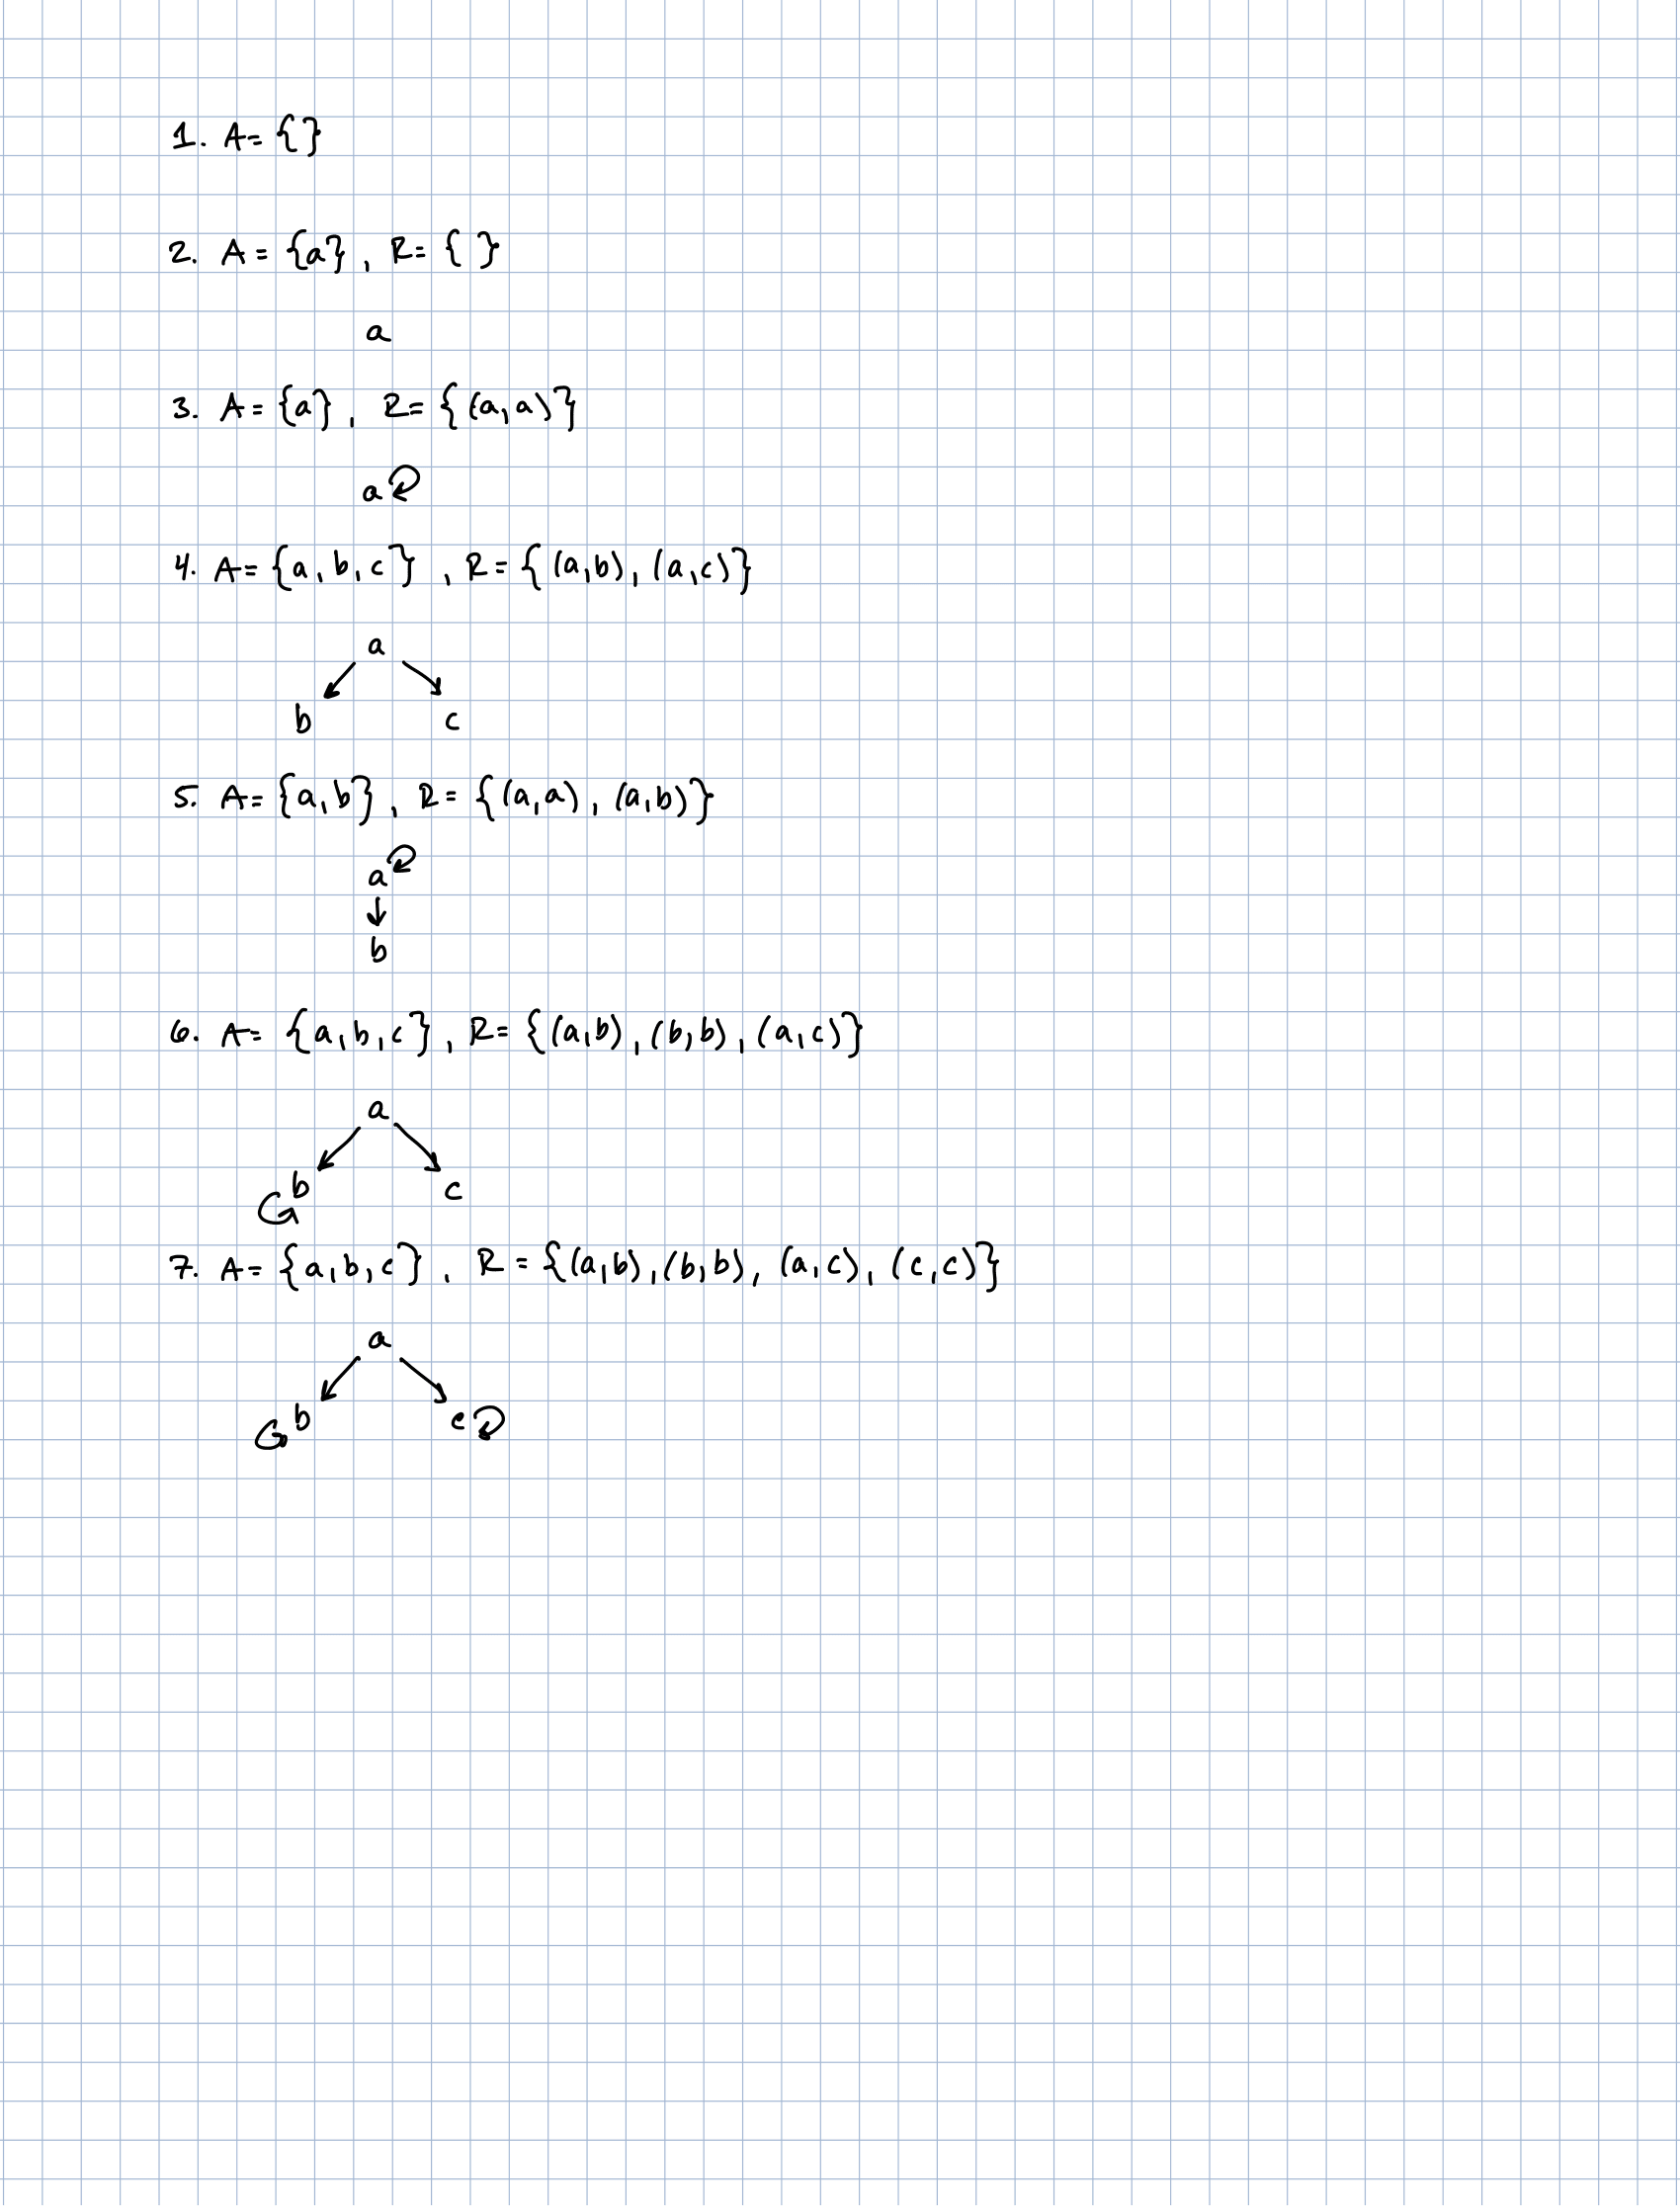
\includegraphics[scale=.75]{CPSC354 HW11-1.png}\\
  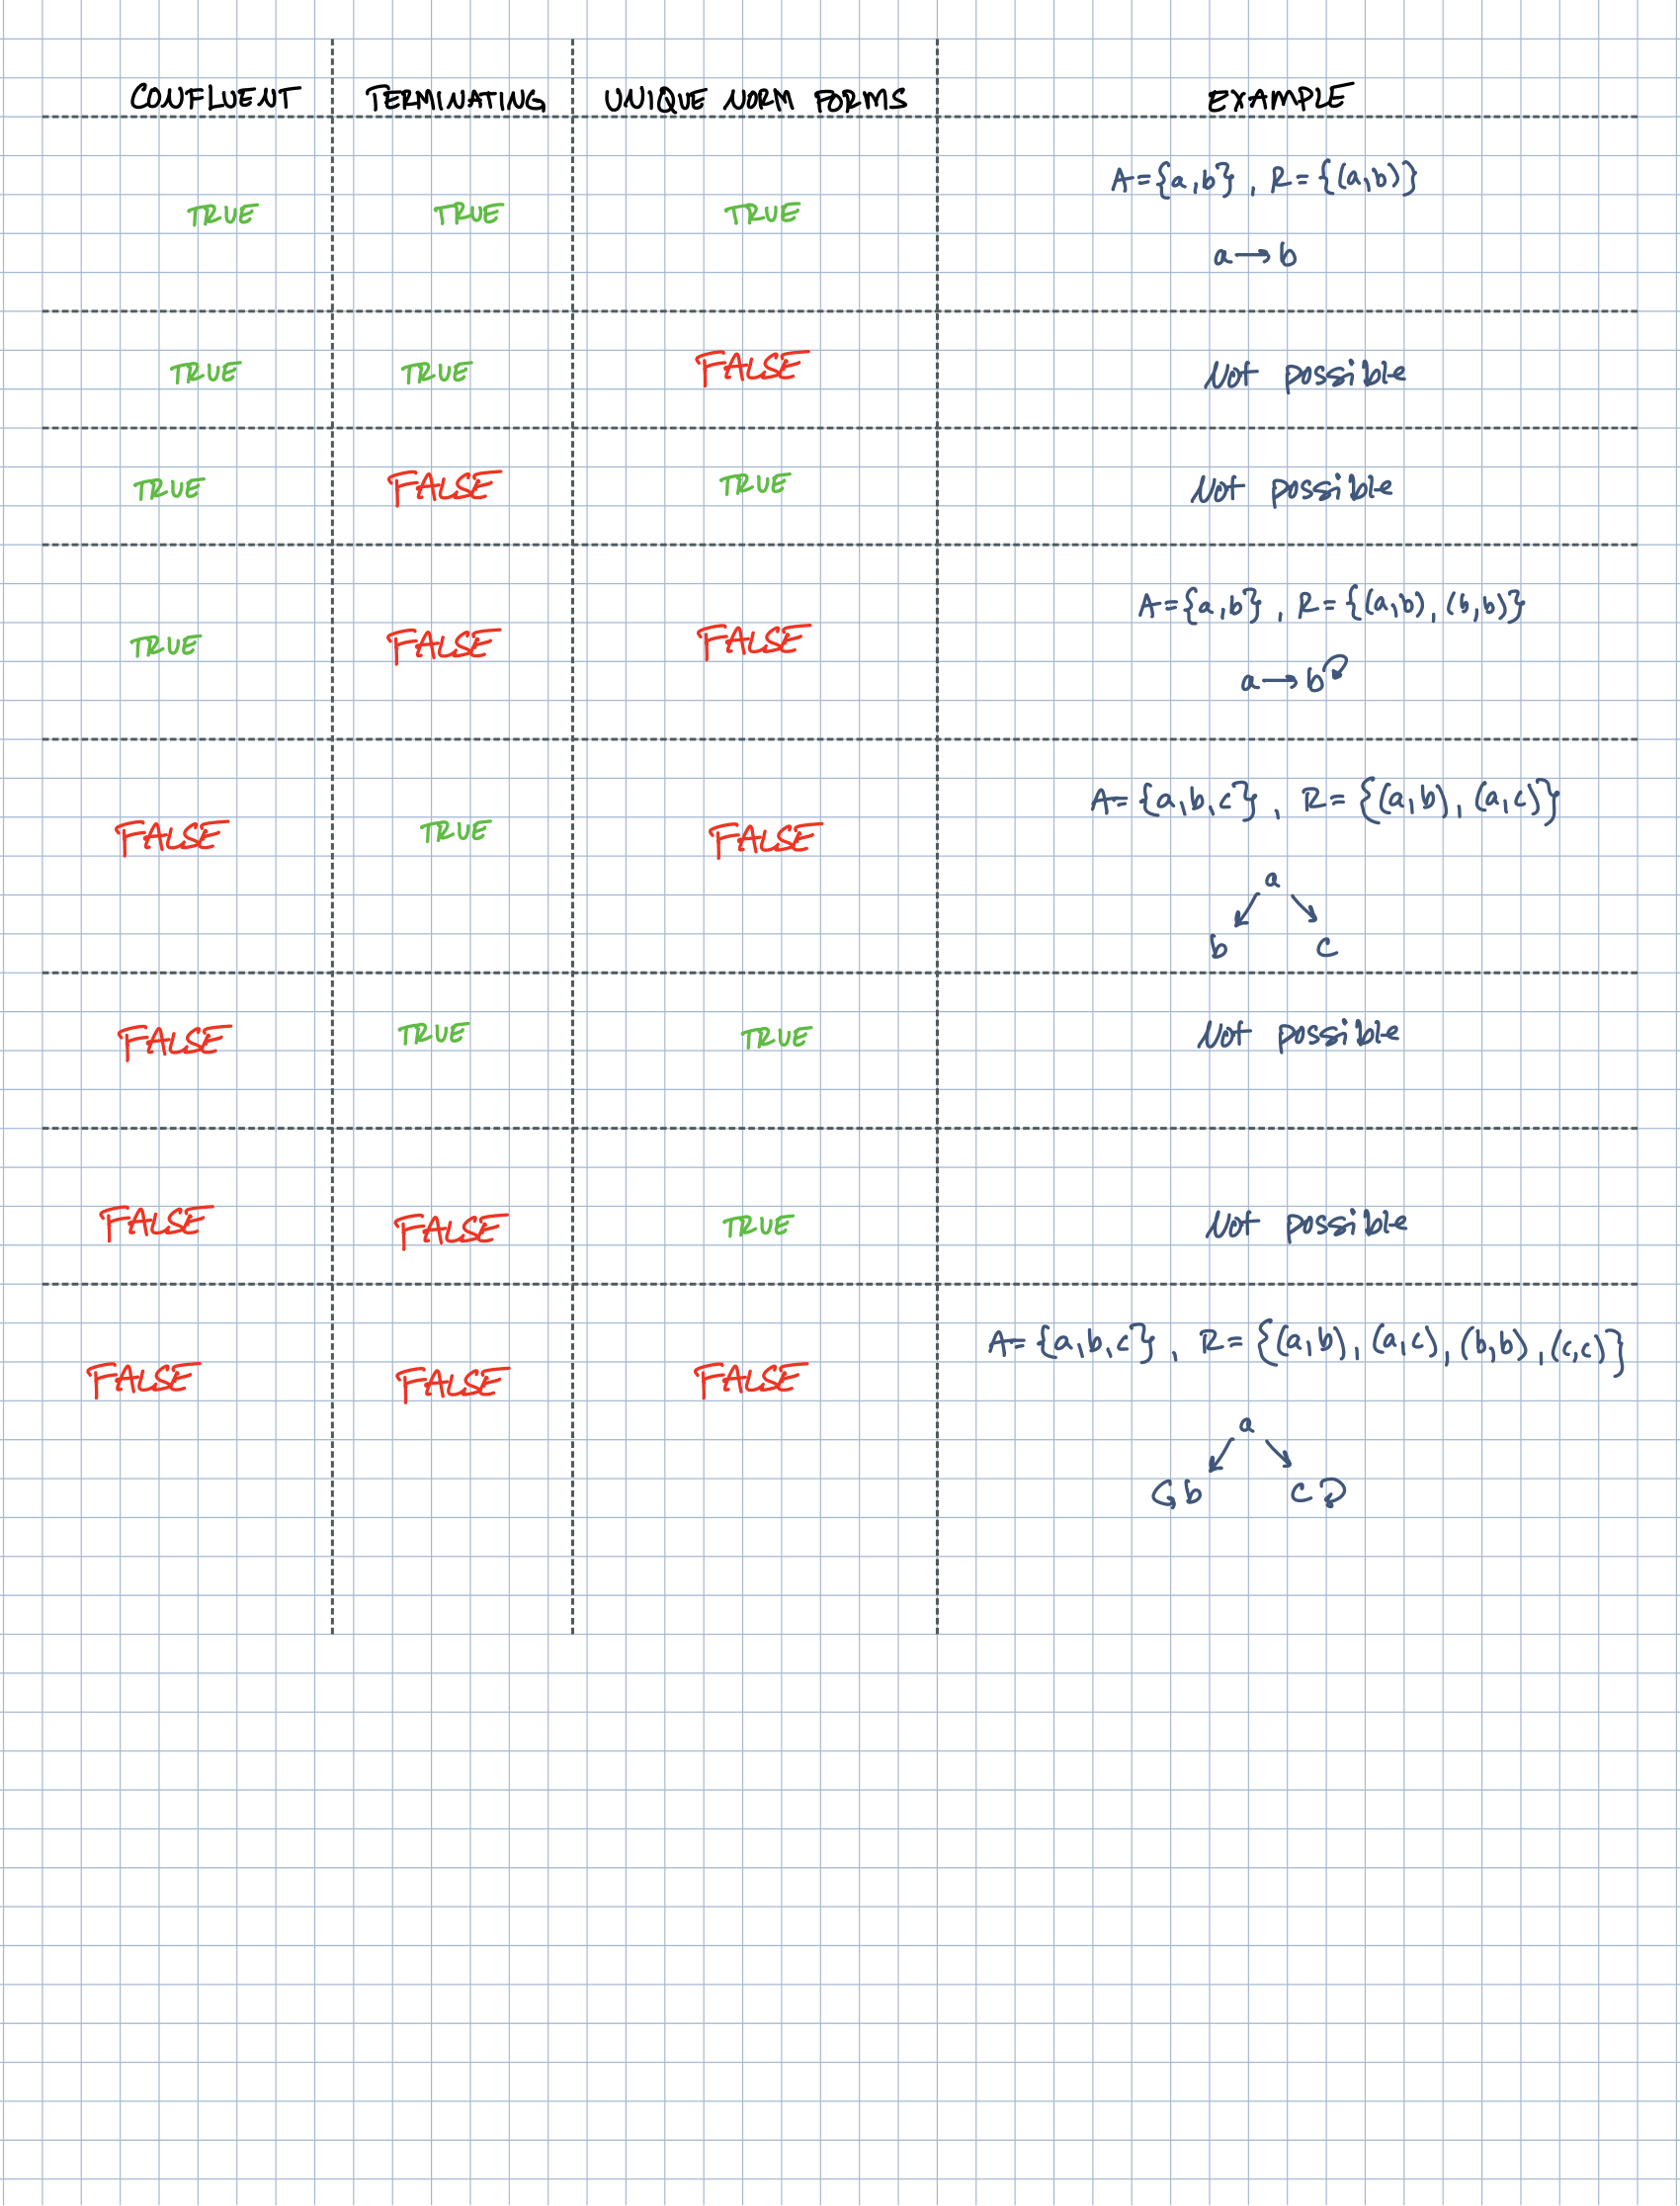
\includegraphics[scale=.75]{CPSC354 HW11-2.png}
  \end{center}

\subsection{Week 12}

\subsubsection*{Notes} This week in class we talked about invariants, specifically within the context of a sliding puzzle on Tuesday. This puzzle was an interesting demonstration of how moving pieces around a puzzle which was impossible to begin with will never make it solvable, and vice versa. This also leads off of the discussion that we had about splitting computations into different equivalence classes, such that the defining characteristics of those computations will always remain regardless of how the system is changed. We discussed fixed-point combinators on Thursday, and how they can be used to implement recursion into lambda calculus. To do this we re-visited conditionals in lambda calculus and defined naming.

\subsubsection*{Question} Are there other methods of performing recursion in lambda calculus besides fixed-point combinators? Does the definition of naming functional or is it just syntactic sugar?

\subsubsection*{Homework}

\[
\begin{aligned}
  \text{ let fact(3)} &\equiv  \text{ ( fix (f.x x)) in 3} &\dashleftarrow\text{def of let rec}\\
  &\equiv\beta\text{ f.x ( fix (f.x x)) in 3} &\dashleftarrow\text{beta rule: sub fix F}\\
  &\equiv\beta\text{ 3 * ( fix (f.x x)) in 2} &\dashleftarrow\text{beta rule: sub fix F}\\
\end{aligned}
\]

\subsection{Week 13}

\subsubsection*{Notes} The linked story in the schedule about Achilles and tortoise was a very fun read, and had some interesting reflections on the termination of systems. If someone must continually accept new premises to justify previous conclusions, then the system will never terminate. In recursion, this endless cycle is handled with a base case, which is compared to at the beginning of each recurse. In the story, it was interesting because as opposed to continually moving toward a solution, Achilles and the tortoise always moved further away from it. In programming, a recursion problem such as fibonacci always moves toward a problem in order to intersect with the base case and therefore terminate. In this way it is interesting that the story described a problem that could not terminate because the tortoise (unreasonably) continually changed the base case.

\subsubsection*{Question} How transferable are heuristics of puzzle solving in real life (i.e. solving in our heads) vs using a computer to solve. Computers use algorithms to solve puzzles (assuming they are solvable), but are there algorithms that are less efficient when performing them in real life?

\subsubsection*{Homework} This week we worked on the next milestone for our interpreter.

\textbf{Exercise 5}\\

(1) Reduce the following strings using the rewrite rules:\\
|    1. $abba \rightarrow aba \rightarrow aa \rightarrow \epsilon$\\
|    2. $bababa \rightarrow baabba \rightarrow bbba \rightarrow bba \rightarrow ba \rightarrow a$

(2) The ARS does not terminate because $ab \rightarrow ba$ and $ab \rightarrow ba$ are cyclic.

(3) There are 3 equivalence classes:\\
|    1. $\epsilon \rightarrow \epsilon$\\
|    2. Even number of $a's \rightarrow \epsilon$\\
|    3. Odd number of $a's \rightarrow a$\\

(4) Yes, either of the following options would work\\
|    1. $ab \rightarrow ba$ becomes $ab \rightarrow a$\\
|    2. $ba \rightarrow ab$ becomes $ba \rightarrow a$\\
These make the ARS terminate without changing the equivalence classes because it does not change the number of $a$s in the string.\\

(5) There are 2 NFs for this ARS, being $\epsilon$ and $a$. The termination strategy in (4) produces an invariant in the number of $a$s in the string.\\

  \textbf{Exercise 5b}\\

  (1) Reduce the following strings using the rewrite rules:\\
    |    1. $abba \rightarrow aba \rightarrow aa \rightarrow a$\\
    |    2. $bababa \rightarrow ababa \rightarrow aaba \rightarrow aaa \rightarrow aa \rightarrow a$

  (2) The ARS does not terminate because $ab \rightarrow ba$ and $ab \rightarrow ba$ are cyclic.

  (3) There are 2 equivalence classes:\\
    |    1. $\epsilon \rightarrow \epsilon$\\
    |    2. Even number of $S \rightarrow a$ where $S$ is any string.\\

  (4) Because the number of $a$s does not matter anymore, we can change either or both of the following rules:\\
    |    1. $ab \rightarrow ba$ becomes $ab \rightarrow a$\\
    |    2. $ba \rightarrow ab$ becomes $ba \rightarrow b$\\
    These make the ARS terminate without changing the equivalence classes because it does not change the number of $a$s in the string.\\

  (5) There are 2 NFs for this ARS, being $\epsilon$ and $a$. The termination strategy in (4) produces an invariant in the number of $a$s in the string.\\

\section{Lessons from the Assignments}

\subsection{Assignment 1}
This was a very fun project and straightforward project to work on, mainly because I could utilize my coding skills with pure python. Without the overhead of needing to understand and organize the baseline code utilized in later assigments, especially with respect to grammars.\\

The specifications for this assignment were straightforward but I was still able to apply some conceptual knowledge towards my solution. The code relies on recursing through parentheses-enclosed statements and evaluating a stack of stored terms. I remember we talked about the value of recursion as a problem-solving tecnique because it encourages a certain way of structuring code (exactly akin to how the evaluate and substitute functions are structured in assignment 3).\\

To this end, let's talk a bit more about the high-level specifications of my solution.
\begin{itemize}
  \item Parsing
    \begin{itemize}
    \item I utilized regex to parse the input string
    \item This separated the string into a sequence of tokens
    \item I allowed for integers, floats, parentheses, and operations
    \end{itemize}
  \item Evaluation
    \begin{itemize}
      \item For each sub-expression (encapsulated within parentheses), the contents are tokenized and then evaluated
      \item One stack contained all values, and another contained all operators
      \item If an operator is encountered
        \begin{itemize}
          \item While the operator at the top of the stack is higher priority than the encountered operator
          \item Two values are popped from the stack and the operator is applied to them
          \item The calculated value is added to the stack
          \item Finally, the encountered operator is added to the stack
        \end{itemize}
      \item This continues until the stacks are empty (when the tokens have all been evaluated)
    \end{itemize}
\end{itemize}

I learned about applying recursion in a dynamic situation without relying on complex behaviour to capture edge cases. This prepared me to take on Assignment 2.\\

\subsection{Assigment 2}
This assignment was our first time utilizing a context free grammar to parse data and evaluate it based on a set of defined contexts. Using a grammar.lark file, we defined a set of rules by which the input would be evaluated. It was interesting to see how type-checking worked via the transformer, and to see that concept reflected in the evaluation.

After we had discussed ASTs in length in class, putting it to use was very cool. I was also very interested in its relation to automata, which I had really enjoyed studying in algorithm analysis. Having an understanding of that concept allowed me to better understand how the context free grammar would be utilized by the transformer.

The specifications of this assignment are not super interesting (compared to Assignment 3), but I will go over them briefly.

\begin{itemize}
  \item Parsing
    \begin{itemize}
      \item The transformer contains definitions for each terminal in the CFG.
      \item These definitions return a tuple with the correct production of concrete syntax.
    \end{itemize}
  \item Evaluation
    \begin{itemize}
      \item Takes in the AST and evaluates it by each terminal syntax.
      \item Correctly produces the expected result of each operation.
    \end{itemize}
\end{itemize}

This assignment taught me about structuring a CFG and, more specifically, about how the transformer inteprets terminal and non-terminal transitions. I thought this was very cool, especially considering how you can structure the grammar to recognize specific syntax, or to pass to another variable (which I read being called "syntactic categories" on Wikipedia).

\subsection{Assignment 3}

Assignment 3 (and continued into assignment 4) is the culmination of the skills and concepts accrued during the class. Our group designed an interpreter to evaluate an AST parsed from a CFG. We constructed the CFG to reflect the required components of the language as well as their nature as operations in concept.

For this assignment, we created a CFG to interpret lambda calculus operations $lam$ and $app$. $Lam$ is an un-typed, anonymous function with a single parameter that receives one argument. The $app$ refers to the application (or injection) of the argument into the function. In our grammar, we recognize lambda expressions as an expression encapsulated in parentheses that demarcated with a backslash ("\textbackslash"). 

The AST is evaluated recursively, and handles each operation singularly (meaning one case at a time). This allows for the recursive function to isolate each operation, which is critical given the AST is (of course) a tree. Our program recognizes the application and expects a lambda to follow. It applies the argument to that expression. 

To evaluate lambda expressions, our program follows these specifications:

\begin{itemize}
  \item Parsing (Grammar \textrightarrow AST)
    \begin{itemize}
      \item The CFG defines terminals for $lam$, $app$, and $var$
      \item These definitions return a tuple with the correct production of concrete syntax
    \end{itemize}
  \item Evaluation
    \begin{itemize}
      \item Recognizes $app$ and finds the enclosed $lam$ operation within its siblings
      \item Evaluates the argument and substitutes (injects) it into the function (following the tecnique of isolating each operation)
    \end{itemize}
\end{itemize}

For this assignment, Szymon and I started by constructing the grammar to produce a valid AST. We evaluated the parsed AST ourselves in order to get the best idea of how to implement the receursive evaluate function. This approach was very valuable, because it allowed us to utilize the skills and concepts we practiced in class, and assure that the evaluate function follows that same logic.

\subsection{Assignment 4}

This assignment is the true culmination of the semester's content and knowledge. Our group implemented an interpreter to handle languages with mathematical and equality-related operations, lambda calculus functions, equality oper, variable naming, if-else-then blocks, recursive lambda functions (following the Y-combinator concept), and handling of multiple programs. 

I was truly excited to work on this assignment, specifically because of my experience on Assignment 2, which was a very fun (and, thankfully, simple) initial dive into implementing interpreted languages. I was excited about writing CFGs to define syntax within a language, and how that model can be extended to account for so many operations. Assignment 4 was my opportunity to really work through how CFGs are written to account for an assortment of different operations in a much more complex context.

\subsubsection{Milestone 1}

The goal of milestone 1 was essentially to take the previous 2 assignments and combine them into one program. 

Since we already had all the necessary grammar and evaluation code to accomplish this milestone, the only challenge lay in integrating them together in the grammar, and then reflecting any necessary changes in the interpreter.py file. 

We noticed that we needed to re-order the syntactic categories. The lower in the grammar a category lies, the higher priority it is (rather, it will be evaluated against first). We made sure that lambda-calculus related operations maintained a higher priority, and that the $app$ terminal maintained the highest priority. Mathematical operations were ordered based on PEMDAS. Expressions within parentheses had a higher priority than $app$ operations, and negatives were above multiplication/division, which were above addition/subtraction. We implemented the necessary functions into the Lark transformer and then implemented handling of each operation in the evaluate function.  

We reused the same implementation of $app$, $lam$, $var$, as well as the mathematical operations. Since each operation is isolated due to recursion, debugging was straightforward and Szymon and I were able to successfully run each test case very quickly. The last thing I will mention about milestone 1 is the use of $number$, which was used in Assignment 3 as well. An evaluation on a $number$ tuple simply returned its enclosed value as a float. 

\subsubsection{Milestone 2}

The purpose of this milestone is to extend the progress from milestone 1 with new operations, including if-else-then blocks and other equality operations, variable naming, and recursive functions.

I thought that implementing $let$ functionality was interesting within the greater context of lambda calculus because it is for anonymous functions. Despite this, $let$ allows us to inject an expression into a lambda function without violating that property. I thought this was cool not only because we maintained that anonymous property, but because it took our language to a higher level, closer to modern languages, and separates the name from its implementation (just like how an abstract class separates the implementation of a class from its behaviour).

Implementing recursion was pretty challenging. Szymon and I needed a couple weeks to properly implement it. The biggest difficulty lay in the grammar, and constructing it in a way that best allows the evaluation to manage the if-else-then block while maintaining arguments. In this way, we wanted to maintain that $fix f$ should evaluate to $f(fix f)$ when applicable. Our confusion lay in navigating the AST and (re)constructing a valid tree from the result of each recurse, with respect to how $lam$ and $app$ need to be parsed into the AST, even if there is no lambda calculus in the function itself.

In the end, the logic for handling recursion follows these specifications:

\begin{itemize}
  \item Evaluate the $let$ expression fully, thereby substituting the function into the body
  \item The expression will always begin with a $fix$
  \item If the $fix$ expression handles a $lam$ operation, restructure the tree to begin with an $app$ (with the appropriate arguments) and evaluate
  \item Fully evaluate, extending the tree until the break condition is met
  \item Recurse through tree until all operations are handled and resolve to the result
\end{itemize}

Equality operations were easy to implement, simply requiring some expression on either side of a "==" or "<=" variable. This is implemented as the native equality comparison of each fully evaluated operand. If-else-then was implemented similarly. We can expect an equality operation as the first expression within an if clause, and therefore the fully evaluated result of that expression (which will always be 1.0 for True, and 0.0 for False) will dictate if we recurse evaluate into the $then$ or $else$ expressions.

\subsubsection{Milestone 3}

The goal of milestone 3 was to implement list and program (sequencing) functionality into our language.

We started by first implementing list functionality. We added the appropriate syntax to our grammar within the second-highest priority syntactic category. For list syntax, we can expect variables, numbers, variable renaming, recursive functions, and encapsulated expressions. Following these expectations, the aforementioned operations are placed in the highest-priority syntactic category. Throughout the grammar, we made sure to always place data type terminals at a higher priority than operation terminals. This made sure that variables would be appropriately interpreted before introducing any operation syntax.

Since we could be sure that any two variables in a list were encapsulated within $cons$, we could layer variables within a list within a chain of $cons$. The implementation of $cons$ allowed that, the evaluation of the first variable will always be the head of the list. If the second variable is a $cons$, then there are other variables in the list, which we can continue to recurse on. Otherwise, we have found tail of the list.

Implementing programs was very straightforward. If we encountered ";;" in the input, we know we must isolate the implementation of each program. In accomplish this, the grammar separates the interpretation of each program. When evaluating, we can fully evaluate each program, and then return the combination of each program result joined by ";;".

\section{Conclusion}\label{conclusion}

This class was a joy to take, and especially to take high level concepts and apply them in meaningful ways. Besides a focus on the technical implementation of programming language interpreters, and the underlying concepts behind how languages are constituted, I enjoyed learning about the history of closely-related logic systems, puzzles and exercises that provide substance to concepts, and thinking about the application of lessons onto my personal areas of interest. I think that the content, and specifically the assignments, provided an invaluable opportunity to practice a very interesting form of development. I had never worked with grammars before, which are very cool, but most of all I have never developed a program quite like interpreter.py. This recursive, operation-based approach was very interesting to wrap my head around, but once I had, extending it came more easily. 

One concept in particular was very interesting, and applicable to my field of interest (being game development). Invariants are properties or conditions that remain true during the course of a program. I immediately drew comparisons to game design, wherein the idea of directives, objectives, and consistent behaviour are paramount. Throughout the course of gameplay, there are systems that must remain consistent, and asserting an invariant can help us maintain that consistency. AI systems, for example, comprise a set of predefined behaviours. While the state of the system can change, the underlying conditions that define those states always remain the same. Conflicting conditions are commonplace in these systems (e.g. in-combat and in-combat-low-health share at least one condition), and yet the underlying invariant comprises a set of conditions and can manage these overlaps.


\begin{thebibliography}{99}
\bibitem[BLA]{bla} Author, \href{https://en.wikipedia.org/wiki/LaTeX}{Title}, Publisher, Year.
\end{thebibliography}

\end{document}
